
The collaboration efforts and the management structure are organized around the objectives of the project, the outcome assessment, and research team expertise. The collaborative effort will extend beyond the scientific research to teaming on testbed development, student supervision and training, and educational activity.

\subsection{Research team members and their expertise}
The research project pools diverse expertise from Illinois Institute of Technology (IIT), Northwestern University, and Rutgers University needed for the successful completion of the proposed interdisciplinary research activity. The project team has a prior history of successful collaborations. The team members and their complementary research expertise are as follows:\\

\textbf{Ashfaq Khokhar (AAK), IIT}, (Routing and MAC Layer in WSN, Data Security, Privacy Preserving Data Mining, Power Efficient Scalable Computing),  

\textbf{Farid Nait-Abdesselam (FN), IIT}, (Wireless Networks, Protocol Security, Data Analytics), 

\textbf{Mubbasir Kapadia (MK), Rutgers University}, (Machine Learning, Computer Vision), 

\textbf{Vladimir Pavlovic (VP), Rutgers University}, (xxx), 

\textbf{Aleksander Kuzamanovic (AK), Northwestern University} (xxx),

\textbf{Goce Trajcevski (GT), Northwestern University}, (Moving Objects Databases, Uncertainty in Mobile Data, Active Databases and Triggers). \\

The PIs involved in this project have a history of research collaboration on jointly funded projects. Dr. Khokhar, Dr. Trajcevski, and Dr. Nait-Abdesselam (then an international partner from France) have collaborated on a Large NeTS-NSF award, have co-advised PhD students, and have co-authored several conference and journal publications. 
\colorbox{red}{ADD OTHERS HERE…}\\
The collaborative effort will extend beyond the scientific research to teaming on testbed development, student supervision and training, course development, workshop organization, and performance evaluation of the technology developed.

\subsection{PI research collaboration} 
If the team awarded the funding, a kick-off meeting will be held within a week of the announcement for all investigators, participating senior research personnel, and graduates students. A broad overview of the research activities will be presented and yearly research targets and deliverables will be set. We will hold biweekly meetings with the attendance of the PIs and Ph.D students from all the campuses. Towards this end we plan to use social media tools such as Google Hangouts and Zoom.

The major research tasks, group interactions, research outcomes, deliverables, and possible applications likely to emerge out of the proposed research are depicted in Figure~\ref{CM-1}. The activities in the four research threads and their linkages are captured in the four rectangular boxes on the left. We will have the following collaborative roles for the PIs in the research activities of the project effort, with the team lead identified in bold:\\

\textbf{Trajcevski}, Kapadia, Pavlovic: Data Processing and Information Modeling 

\textbf{Pavlovic}, Khokhar, Kuzmanovic, Nait-Abdesselam: Data Analytics

\textbf{Kuzmanovic}, Khokhar, Nait Abdesselam: Security and Proivacy

\textbf{Nait-Abdesselam}, Kapadia, Trajcevski: Testbed Implementation and Validation \\

These roles are also identified (with the abbreviations of their first and last names) as white ovals in Figure~\ref{CM-1}. Also, we envision realization of the objectives defined for the research activities will produce three outcome components (i) Efficient IoT Representations, (ii) Privacy Preserving Data Analytics, and (iii) Private Secure Connectivity among heterogeneous devices and users. These in turn will be assembled into the overall deliverable of comprehensive software system and testbed for realizing Dynamic Data Driven Cyber Human Networks consisting of IoT avatars. Research in all key areas will proceed in parallel and overlapping phases, and the planned progress over a three-year timeline is shown in quarters at the bottom in Figure~\ref{CM-1}. 

\begin{wrapfigure}{R}{0.70\textwidth} \vspace{-3mm}
	\centerline{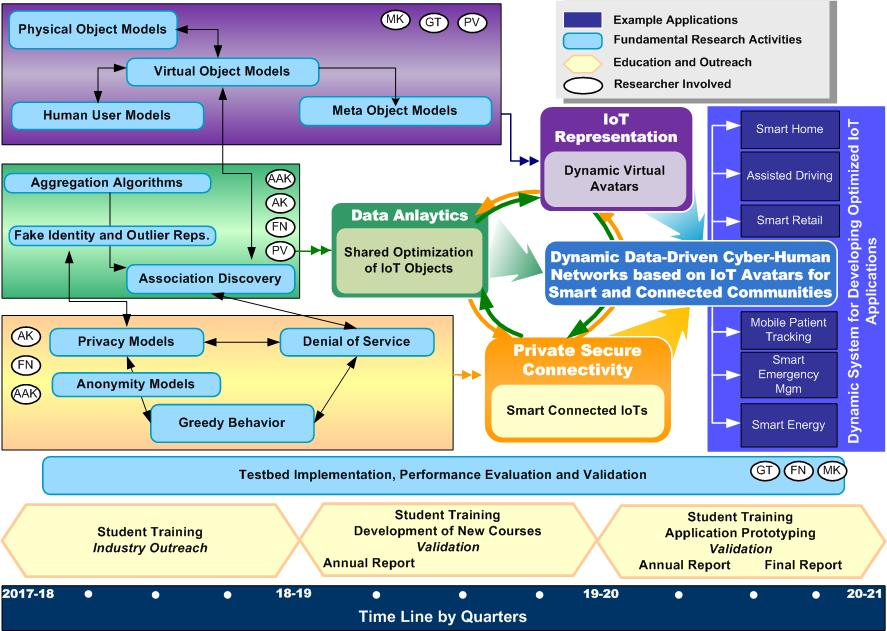
\includegraphics[width=0.61\textwidth]{./Timeline-v1.jpg}}
	\vspace{-3mm} \caption{Relationship of major research tasks, group interactions, research outcomes, deliverables, and possible applications likely to emerge out of the proposed research}
	\label{CM-1}
	\vspace{-3mm}
\end{wrapfigure}

The management structure is organized around the main research themes identified in Section 4.  Prof. Khokhar will assume overall responsibility for coordination of research activity. He will be in regular contact with the other investigators and personnel. He has extensive experience in managing large domestic and international teams and has organized NSF-sponsored workshops. The progress of then project will be monitored by a Project Steering Committee, consisting of one Co-PI from each institution. Three working groups will oversee the research on the main research threads described in the proposal, and will be responsible for assessing the research outcomes. Due to the need for collaborative work on the research activities, each investigator will serve on at least two of the three working groups.


\subsection{PI research collaboration and student supervision} 
Upon the award of the project, a kick-off meeting will be held within a week of the announcement for all investigators, participating senior research personnel, and graduates students. A broad overview of the research activities will be presented and yearly research targets and deliverables will be set. We will hold monthly cross-institutional and bi-weekly intra-institutional meetings with the attendance of the PIs and Ph.D students. 

In the first eight quarters, the proposed research activity will include participation of \textit{one postdoc and three graduate students} supported by the project and several undergraduate students carrying out Honors College activity. During the last eight quarters, the project will support \textit{seven graduate students and a Post-doctoral} researcher. The students will receive research training in diverse emerging topics such as Information abstraction, data analytics, and robust privacy and security of networks and its components. Since the work requires collaboration beyond the immediate field of interest, the students will be co-supervised by faculty from participating institutions and will gain extensive experience in inter-disciplinary research activity.

\subsection{Dissemination plan} 
A project website will be established to disseminate the results and the code developed during the project. We will organize at least one workshops in a leading conference on IoTs promote our research among peers working on related research issues. In addition we will work to organize special issues of journals on these topics. The travel cost budgeted in the proposal is related to these dissemination activities

\subsection{Management of testbed development and technology transfer} 
The protocols and techniques developed in this project will be evaluated using an experimental testbed consisting of a network of IoT devices. This effort will be managed jointly by Dr. Khokhar and Dr. Trajcevski. Furthermore multiple commercial organizations working the domain of smart sensor systems and applications has indicated strong interest in the proposed project. For additional details please we refer to the letters of collaboration uploaded as single copy documents.
